\documentclass[class=article, crop=false]{standalone}
\usepackage[margin=1in]{geometry}
\usepackage[linesnumbered,ruled,vlined]{algorithm2e}
\usepackage{amsfonts}
\usepackage{amsmath}
\usepackage{amssymb}
\usepackage{amsthm}
\usepackage{enumitem}
\usepackage{fancyhdr}
\usepackage{hyperref}
\usepackage{minted}
\usepackage{multicol}
\usepackage{pdfpages}
\usepackage{standalone}
\usepackage[many]{tcolorbox}
\usepackage{tikz-cd}
\usepackage{transparent}
\usepackage{xcolor}
% \tcbuselibrary{minted}

\author{Nathan Solomon}

\newcommand{\fig}[1]{
    \begin{center}
        \includegraphics[width=\textwidth]{#1}
    \end{center}
}

% Math commands
\renewcommand{\d}{\mathrm{d}}
\DeclareMathOperator{\id}{id}
\DeclareMathOperator{\im}{im}
\DeclareMathOperator{\proj}{proj}
\DeclareMathOperator{\Span}{span}
\DeclareMathOperator{\Tr}{Tr}
\DeclareMathOperator{\tr}{tr}
\DeclareMathOperator{\ad}{ad}
\DeclareMathOperator{\ord}{ord}
%%%%%%%%%%%%%%% \DeclareMathOperator{\sgn}{sgn}
\DeclareMathOperator{\Aut}{Aut}
\DeclareMathOperator{\Inn}{Inn}
\DeclareMathOperator{\Out}{Out}
\DeclareMathOperator{\stab}{stab}

\newcommand{\N}{\ensuremath{\mathbb{N}}}
\newcommand{\Z}{\ensuremath{\mathbb{Z}}}
\newcommand{\Q}{\ensuremath{\mathbb{Q}}}
\newcommand{\R}{\ensuremath{\mathbb{R}}}
\newcommand{\C}{\ensuremath{\mathbb{C}}}
\renewcommand{\H}{\ensuremath{\mathbb{H}}}
\newcommand{\F}{\ensuremath{\mathbb{F}}}

\newcommand{\E}{\ensuremath{\mathbb{E}}}
\renewcommand{\P}{\ensuremath{\mathbb{P}}}

\newcommand{\es}{\ensuremath{\varnothing}}
\newcommand{\inv}{\ensuremath{^{-1}}}
\newcommand{\eps}{\ensuremath{\varepsilon}}
\newcommand{\del}{\ensuremath{\partial}}
\renewcommand{\a}{\ensuremath{\alpha}}

\newcommand{\abs}[1]{\ensuremath{\left\lvert #1 \right\rvert}}
\newcommand{\norm}[1]{\ensuremath{\left\lVert #1\right\rVert}}
\newcommand{\mean}[1]{\ensuremath{\left\langle #1 \right\rangle}}
\newcommand{\floor}[1]{\ensuremath{\left\lfloor #1 \right\rfloor}}
\newcommand{\ceil}[1]{\ensuremath{\left\lceil #1 \right\rceil}}
\newcommand{\bra}[1]{\ensuremath{\left\langle #1 \right\rvert}}
\newcommand{\ket}[1]{\ensuremath{\left\lvert #1 \right\rangle}}
\newcommand{\braket}[2]{\ensuremath{\left.\left\langle #1\right\vert #2 \right\rangle}}

\newcommand{\catname}[1]{{\normalfont\textbf{#1}}}

\newcommand{\up}{\ensuremath{\uparrow}}
\newcommand{\down}{\ensuremath{\downarrow}}

% Custom environments
\newtheorem{thm}{Theorem}[section]

\definecolor{probBackgroundColor}{RGB}{250,240,240}
\definecolor{probAccentColor}{RGB}{140,40,0}
\newenvironment{prob}{
    \stepcounter{thm}
    \begin{tcolorbox}[
        boxrule=1pt,
        sharp corners,
        colback=probBackgroundColor,
        colframe=probAccentColor,
        borderline west={4pt}{0pt}{probAccentColor},
        breakable
    ]
    \color{probAccentColor}\textbf{Problem \thethm.} \color{black}
} {
    \end{tcolorbox}
}

\definecolor{exampleBackgroundColor}{RGB}{212,232,246}
\newenvironment{example}{
    \stepcounter{thm}
    \begin{tcolorbox}[
      boxrule=1pt,
      sharp corners,
      colback=exampleBackgroundColor,
      breakable
    ]
    \textbf{Example \thethm.}
} {
    \end{tcolorbox}
}

\definecolor{propBackgroundColor}{RGB}{255,245,220}
\definecolor{propAccentColor}{RGB}{150,100,0}
\newenvironment{prop}{
    \stepcounter{thm}
    \begin{tcolorbox}[
        boxrule=1pt,
        sharp corners,
        colback=propBackgroundColor,
        colframe=propAccentColor,
        breakable
    ]
    \color{propAccentColor}\textbf{Proposition \thethm. }\color{black}
} {
    \end{tcolorbox}
}

\definecolor{thmBackgroundColor}{RGB}{235,225,245}
\definecolor{thmAccentColor}{RGB}{50,0,100}
\renewenvironment{thm}{
    \stepcounter{thm}
    \begin{tcolorbox}[
        boxrule=1pt,
        sharp corners,
        colback=thmBackgroundColor,
        colframe=thmAccentColor,
        breakable
    ]
    \color{thmAccentColor}\textbf{Theorem \thethm. }\color{black}
} {
    \end{tcolorbox}
}

\definecolor{corBackgroundColor}{RGB}{240,250,250}
\definecolor{corAccentColor}{RGB}{50,100,100}
\newenvironment{cor}{
    \stepcounter{thm}
    \begin{tcolorbox}[
        enhanced,
        boxrule=0pt,
        frame hidden,
        sharp corners,
        colback=corBackgroundColor,
        borderline west={4pt}{0pt}{corAccentColor},
        breakable
    ]
    \color{corAccentColor}\textbf{Corollary \thethm. }\color{black}
} {
    \end{tcolorbox}
}

\definecolor{lemBackgroundColor}{RGB}{255,245,235}
\definecolor{lemAccentColor}{RGB}{250,125,0}
\newenvironment{lem}{
    \stepcounter{thm}
    \begin{tcolorbox}[
        enhanced,
        boxrule=0pt,
        frame hidden,
        sharp corners,
        colback=lemBackgroundColor,
        borderline west={4pt}{0pt}{lemAccentColor},
        breakable
    ]
    \color{lemAccentColor}\textbf{Lemma \thethm. }\color{black}
} {
    \end{tcolorbox}
}

\definecolor{proofBackgroundColor}{RGB}{255,255,255}
\definecolor{proofAccentColor}{RGB}{80,80,80}
\renewenvironment{proof}{
    \begin{tcolorbox}[
        enhanced,
        boxrule=1pt,
        sharp corners,
        colback=proofBackgroundColor,
        colframe=proofAccentColor,
        borderline west={4pt}{0pt}{proofAccentColor},
        breakable
    ]
    \color{proofAccentColor}\emph{\textbf{Proof. }}\color{black}
} {
    \qed \end{tcolorbox}
}

\definecolor{noteBackgroundColor}{RGB}{240,250,240}
\definecolor{noteAccentColor}{RGB}{30,130,30}
\newenvironment{note}{
    \begin{tcolorbox}[
        enhanced,
        boxrule=0pt,
        frame hidden,
        sharp corners,
        colback=noteBackgroundColor,
        borderline west={4pt}{0pt}{noteAccentColor},
        breakable
    ]
    \color{noteAccentColor}\textbf{Note. }\color{black}
} {
    \end{tcolorbox}
}


\fancyhf{}
\lhead{Nathan Solomon}
\rhead{Page \thepage}
\pagestyle{fancy}

\begin{document}
\section{5/24/2024 lecture}
\subsection{Silicon-based life forms}
Silicon is similar to carbon in that it can form four bonds, but those bonds are slightly weaker. Silicon doesn't form double bonds as easily, which limits the variety of molecules it can form. Carbon is also a bit more useful to life than silicon because $CO_2$ is a fluid, so it can move around easily, but $SiO_2$ (sometimes called silica or dilicon dioxide) is a solid -- in fact, we see it in quartz, sand, and glass.
\begin{note}
    Lots of people confuse the metalloid silicon with silicone, which is a family of organic polymers. Rubbery silicone is often used in breast implants and heat-resistant spatulas, whereas silicon is essential for microchips because we can make p-type and n-type semiconductors by doping the silicon.
\end{note}
\par
Since silicon is a thousand times as abundant in the Earth's crust as carbon is, we can assume that carbon-based life arises more easily than silicon-based life.
\subsection{Proteins}
The main ``building blocks of life" are
\begin{itemize}
    \item Carbohydrates
    \item Lipids
    \item Proteins
    \item Nucleic acids
\end{itemize}
Here's a saturated triglyceride, which is a common example of a lipid:

\begin{center}
    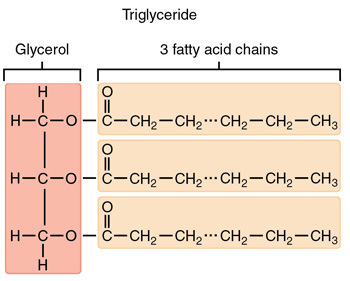
\includegraphics[width=.6\textwidth]{triglycerides.jpg}
\end{center}
\begin{note}
    If the fatty acids there weren't saturated with hydrogen, they wouldn't form straight rigid lines, so it would be less stiff. Adding hydrogen turns vegetable oil into shortening. Typically, saturated fats are worse for your health, because they can clog arteries.
\end{note}
Out of all of those proteins are the most interesting because they can serve several puposes. The main types are enzymes (which catalyze reactions), structural proteins, transport proteins (which move other molecules), muscle proteins (which contract when they receive an electrical signal), and signaling proteins (some types of hormones are proteins). There are also healing proteins, like fibrogen and antibodies, nutrient storage proteins (like egg whites), and toxins (like botox).
\par
Proteins are made from 20 types of amino acids which link via dehydration bonds. Each amino acid is made of an amino group ($NH_2$), a carboxyl group ($COOH$), a central $CH$, and a unique side chain connected to the central $CH$. When they bond, an $H$ falls off the amino group and an $OH$ falls off the carboxyl group.
\subsection{Chirality}
Chircality can determine the effect of a molecule, and we can assume that all life which shares a common origin will have the same handedness.
\par
All life on Earth uses a left-handed form of the amino acid alanine. We believe that all life on Earth descended from a common ancestor, and the last common ancestor, called LUCA, existed 3.5-3.8 billion years ago.
\subsection{Metabolism}
All life forms can be classified as heterotrophs or autotrophs. Those who get a majority of their carbon by consuming food are heterotrophs -- this includes all animals. Organisms that get their carbon from their environment in other ways, like photosynthesis or chemosynthesis, are autotrophs.
\par
In addition to classifying organisms as ``hetero-" or ``auto-" based on how they get carbon, we classify them as ``photo-" or ``chemo-" based on where they get their energy. Animals are chemoheterotrophs and plants are photoautotrophs.
\par
Liquid water is essential for metabolism because it enables aqueous reaction, transports essential chemicals, among other things.

\end{document}
